\documentclass[11pt,a4paper]{article}

% ── Packages ──────────────────────────────────────────────────────────
\usepackage[utf8]{inputenc}
\usepackage[T1]{fontenc}
\usepackage{microtype}
\usepackage{graphicx}
\usepackage{booktabs}
\usepackage{amsmath,amssymb}
\usepackage{hyperref}
\usepackage{enumitem}
\usepackage[margin=1in]{geometry}
\usepackage{xcolor}
\usepackage{multirow}
\usepackage{array}
\usepackage{caption}
\usepackage{tikz}
\usetikzlibrary{arrows.meta,positioning,fit}

\definecolor{darkblue}{RGB}{0,70,140}
\hypersetup{colorlinks,linkcolor=darkblue,citecolor=darkblue,urlcolor=darkblue}

% ── Title ─────────────────────────────────────────────────────────────
\title{\textbf{HMC-Torch: A Modular Platform for Hierarchical Multi-Label
Classification\\ with R-Matrix Constraints}}

\author{
  Bruno Sette\textsuperscript{1} \\
  \textsuperscript{1} Federal University of São Carlos (UFSCar), Brazil \\
  \texttt{brunosilvasette@gmail.com}
}

\date{August 2026}

\begin{document}
\maketitle

% ── Abstract ──────────────────────────────────────────────────────────
\begin{abstract}
We present \textsc{hmc-torch}, a modular and extensible platform for
Hierarchical Multi-Label Classification (HMC) that integrates the
R-matrix constraint---originally proposed by Giunchiglia \&
Lukasiewicz (2018, NeurIPS)---as a first-class architectural
component. The framework separates data contracts
(\texttt{DatasetBundle}, \texttt{Hierarchy}), feature encoders, and
reusable HMC heads, enabling reproducible experimentation across 28
datasets spanning tree and DAG hierarchies. We report
\textbf{new state-of-the-art} on ArXiv, WOS, and AAPD, competitive
baselines on FunCat and EUR-Lex 57K, and a sparse R-matrix formulation
that preserves hierarchical consistency in $O(C{+}E)$ memory. On 9 Gene
Ontology datasets, sparse reconciliation improves AUPRC on every
dataset while avoiding the dense $O(C^2)$ matrix, which exceeds GPU
memory at this scale.

\smallskip
\noindent\textbf{Availability:} \url{https://github.com/sette/hmc-torch} \textbar{}
\url{https://pypi.org/project/hmc-torch/}
\end{abstract}

% ═══════════════════════════════════════════════════════════════════════
\section{Introduction}
% ═══════════════════════════════════════════════════════════════════════

Hierarchical Multi-Label Classification (HMC) is a structured
prediction task where each instance is assigned to one or more nodes
in a predefined class hierarchy (tree or DAG). HMC arises naturally in
scientific domains: categorizing academic papers into topic taxonomies
(ArXiv, WOS), annotating proteins with Gene Ontology (GO) terms, and
classifying diatoms into morphological hierarchies.

The HMC literature has produced increasingly sophisticated
methods---from local per-level classifiers~\cite{silla2011hmc} to
global approaches with graph neural networks~\cite{zhou2020hiagm} and
ontology representation learning~\cite{www2022ontology}. A key
architectural innovation was introduced by Giunchiglia \&
Lukasiewicz~\cite{giunchiglia2018hmc}: the \textbf{R-matrix}
(ancestor closure matrix) that enforces hierarchical consistency by
ensuring every parent node's predicted probability is at least as
large as its children's. However, this constraint has typically been
applied as a post-processing step or embedded within complex recurrent
architectures, limiting its adoption and systematic study.

We present \textsc{hmc-torch}, a platform that elevates the R-matrix
from a post-hoc correction to a \textbf{first-class architectural
component}, integrated during both training (via consistency loss) and
inference (via bottom-up reconciliation). Our design follows three
principles:

\begin{enumerate}[leftmargin=*,nosep]
  \item \textbf{Separation of concerns.} Data contracts
    (\texttt{DatasetBundle}, \texttt{Split}) decouple dataset loading
    from model training. Feature encoders follow a common
    \texttt{fit/transform} protocol across modalities.
  \item \textbf{Explicit hierarchy modeling.} Tree-structured
    (FunCat) and DAG-structured (Gene Ontology) hierarchies are
    distinct types with type-specific reconciliation, preventing
    silent conflation of single-parent and multi-parent semantics.
  \item \textbf{R-matrix as infrastructure.} The ancestor closure
    matrix is a reusable, differentiable layer available to any
    downstream head, enabling systematic ablation studies of its
    contribution.
\end{enumerate}

Throughout the paper, we use \textbf{dense R-matrix} for the explicit
$C \times C$ ancestor-closure matrix, \textbf{R-matrix constraint} for
the hierarchical consistency property itself, and \textbf{sparse
R-matrix formulation} for the graph-based version that preserves the
same semantics without materializing the dense matrix.

Our contributions are:
\begin{itemize}[leftmargin=*,nosep]
  \item A modular HMC platform supporting 28 datasets across 7
    domains, with reproducible experiment manifests and a shared
    encoder/head interface.
  \item \textbf{New SOTA on ArXiv, WOS, and AAPD} using frozen or
    fine-tuned SPECTER2 with the R-matrix constraint.
  \item \textbf{Sparse R-matrix formulation}: a graph-based
    $O(C{+}E)$ formulation that enforces the same constraint on large
    DAGs without materializing the dense matrix.
  \item Competitive FunCat performance with simpler models, plus an
    explicit analysis of where the R-matrix is insufficient relative
    to ontology-based methods.
  \item Open-source release with GPU acceleration and reproducible
    experiment artifacts.
\end{itemize}

% ═══════════════════════════════════════════════════════════════════════
\section{Related Work}
% ═══════════════════════════════════════════════════════════════════════

\subsection{HMC Methods}

Early HMC approaches treated each level independently with local
classifiers~\cite{silla2011hmc,cerri2014hmc}. Global methods predict
all classes jointly:~\cite{weihs2018hmc} proposed a flat multi-label
classifier with post-hoc constraint propagation, while~\cite{zhou2020hiagm}
introduced HiAGM, combining a text encoder with a Graph Convolutional
Network (GCN) over the label hierarchy. HTC-infoMAX~\cite{htcinfomax}
added mutual information maximization. For protein function prediction
(FunCat/GO benchmarks),~\cite{www2022ontology} proposed ontology
representation learning, achieving state-of-the-art AUPRC by jointly
learning class embeddings from the GO hierarchy structure.

For tabular/genomic data, CLUS-HMC~\cite{clus} uses decision trees
with hierarchical constraints, while HMCN~\cite{giunchiglia2018hmc}
propagates information across hierarchy levels via recurrent
architectures and introduced the R-matrix constraint that we build
upon.

\subsection{The R-Matrix Constraint}

The R-matrix (ancestor/closure matrix) is an $N \times N$ binary
matrix where $R_{ij} = 1$ iff class $i$ is an ancestor of class $j$
(including $i=j$). It was introduced by~\cite{giunchiglia2018hmc} as
a post-processing step in the HMCN architecture to enforce
hierarchical consistency: $\forall (i,j): \text{ancestor}(i,j)
\implies p_i \geq p_j$.  Subsequent work~\cite{zhou2020hiagm,
htcinfomax, www2022ontology} adopted similar constraint mechanisms,
but the R-matrix remained tightly coupled to specific architectures.

Our contribution is \textbf{not} the R-matrix itself---we credit
Giunchiglia \& Lukasiewicz (2018) for the original idea---but rather
its elevation to a \textbf{reusable, modular component} within a
general-purpose HMC platform. By making the R-matrix a first-class
abstraction available to any encoder/head combination, we enable
systematic study of its contribution across datasets, modalities, and
architectures.

\subsection{Modular ML Platforms}

Frameworks like HuggingFace Transformers and PyTorch Lightning have
demonstrated the value of modular, composable architectures. However,
HMC-specific platforms remain scarce. The \texttt{hmc-torch} package
fills this gap with HMC-native abstractions and a clear attribution of
which ideas are novel (platform design, systematic evaluation) vs.\
inherited (R-matrix constraint, transformer encoders).

% ═══════════════════════════════════════════════════════════════════════
\section{The HMC-Torch Methodology}
% ═══════════════════════════════════════════════════════════════════════

We present \textsc{hmc-torch} as a methodology built on three
principles: (1) \textbf{strict separation of concerns} via typed data
contracts, (2) \textbf{hierarchy-aware modeling} where the class
taxonomy is a first-class architectural component, not a
post-processing afterthought, and (3) \textbf{modality-agnostic
design} where the same pipeline accommodates text, tabular, image, and
sequence data through a common encoder protocol.

\subsection{Data Contracts: The Foundation}

The central abstraction is the \texttt{DatasetBundle}, which
encapsulates everything a model needs to know about a dataset:

\begin{enumerate}[leftmargin=*,nosep]
  \item \textbf{\texttt{Split}}. One data partition (train, valid, or
    test) containing a feature matrix $X \in \mathbb{R}^{N \times D}$,
    a binary label matrix $Y \in \{0,1\}^{N \times C}$ (where $C$ is
    the total number of class nodes), per-level local label vectors
    $Y_{\text{local}} = [\mathbf{y}^{(0)}, \ldots, \mathbf{y}^{(L-1)}]$
    for $L$ hierarchy levels, and optional sample identifiers for
    deduplication auditing.
  \item \textbf{\texttt{Hierarchy}}. An explicit representation of the
    class taxonomy as either a \texttt{TreeHierarchy} (single-parent,
    FunCat-style) or a \texttt{DagHierarchy} (multi-parent, Gene
    Ontology-style).  Both expose a uniform interface: \texttt{nodes},
    \texttt{levels}, \texttt{node\_index}, \texttt{parents(child)},
    \texttt{children(parent)}, \texttt{ancestors(node)}, and the
    \texttt{r\_matrix} (ancestor closure).  Making the hierarchy type
    explicit prevents the common error of applying tree-specific logic
    to DAG-structured problems.
  \item \textbf{\texttt{FeatureMetadata}}. Describes the feature
    modality (tabular, text, vision, protein, expression), input
    dimensionality, missing value status, sparsity, and whether raw
    data is available for end-to-end training.
\end{enumerate}

This contract-based design enforces a clean boundary between data
loading and model training.  Any dataset adapter (ARFF parser, JSONL
reader, HDF5 loader) must produce a \texttt{DatasetBundle}; any model
must consume one.  This eliminates the ad-hoc data handling that
plagues most HMC implementations and enables the systematic
cross-dataset comparison in Section~\ref{sec:results}.

\subsection{Feature Encoders: One Protocol, Many Modalities}

All feature encoding follows a two-method protocol:

\begin{center}
\texttt{encoder.fit(train\_split)} $\rightarrow$
\texttt{encoder.transform(any\_split)} $\rightarrow$
\texttt{EncodedSplit}
\end{center}

The \texttt{fit} method learns parameters exclusively from the
training split (scaler statistics, imputation values, feature
selection masks).  The \texttt{transform} method applies the fitted
transformation to any split, returning a new \texttt{Split} with
encoded features.  This protocol is \textbf{stateless by
construction}: the same fitted encoder can be serialized, shared, and
applied to new data without leakage.

Current implementations span the major HMC modalities:

\begin{itemize}[leftmargin=*,nosep]
  \item \textbf{Tabular} (\texttt{TabularFeatureEncoder}).  Handles
    missing value imputation (mean), standardization (zero mean, unit
    variance), and optional feature selection via variance threshold
    or mutual information with the label matrix.  For datasets with
    $>$500 features, variance-based filtering removes near-constant
    columns; mutual information selects the top-$K$ most
    label-informative features.
  \item \textbf{Text} (\texttt{TextFeatureEncoder}).  Wraps a
    HuggingFace transformer (SPECTER2-base by default) with CLS-pooling
    for document-level representations.  Supports both frozen
    embeddings (fast, 768-dim output) and fine-tuned mode where
    transformer weights are updated end-to-end with the HMC head.
    Raw-text availability is detected from \texttt{FeatureMetadata};
    if only pre-extracted features exist, the encoder passes through
    unchanged.
  \item \textbf{Protein} (\texttt{ProteinFeatureEncoder}, placeholder).
    Designed for ESM-2 embeddings of amino acid sequences, cached
    per-sequence with model version hashing.  Activated only when raw
    sequences are confirmed available for \texttt{seq\_FUN}.
  \item \textbf{Vision} (\texttt{VisionFeatureEncoder}, placeholder).
    Targets DINOv2/ConvNeXt backbones for Diatoms and ImCLEF image
    data.  Falls back to pre-extracted ARFF features when raw images
    are unavailable.
\end{itemize}

This protocol means that \textbf{any encoder works with any head}:
a tabular model can be swapped for a text transformer without
modifying the downstream HMC architecture.

\subsection{Hierarchical Classification Heads}

The platform provides three head architectures, all producing
\texttt{node\_scores} of shape $(B, C)$ regardless of internal
structure:

\begin{itemize}[leftmargin=*,nosep]
  \item \textbf{GlobalSigmoidHead}. A shared multi-layer perceptron
    over all $C$ class nodes: $\text{MLP}(\mathbf{x}) \rightarrow
    \sigma(\cdot) \rightarrow [0,1]^C$.  This is the simplest and most
    widely applicable head, used in all our experiments except where
    noted.
  \item \textbf{LocalLevelHead}. One independent MLP per hierarchy
    level, each predicting only the classes at that depth:
    $\text{MLP}_\ell(\mathbf{x}) \rightarrow [0,1]^{C_\ell}$.  Trained
    jointly with per-level BCE loss.  Level predictions are assembled
    into a global score vector via the \texttt{to\_global} method using
    the hierarchy's node index mapping.
  \item \textbf{TreePathHead}. For strictly tree-structured tasks
    where each sample follows exactly one root-to-leaf path.  Uses
    masked softmax at each level, where the mask restricts choices to
    children of the parent node chosen at the previous level.  This
    enforces mutual exclusivity within sibling groups.
\end{itemize}

\subsection{R-Matrix: The Hierarchical Constraint Layer}

The R-matrix, introduced by~\cite{giunchiglia2018hmc}, is the
centrepiece of our hierarchical modeling.  Given the class hierarchy
adjacency matrix $A$ (where $A_{ij}=1$ if $i$ is a direct child of
$j$), we compute the transitive closure:

\begin{equation}
R_{ij} = \begin{cases}
1 & \text{if } i = j \text{ or } \exists \text{ path } j \rightarrow \ldots \rightarrow i \text{ in } A \\
0 & \text{otherwise}
\end{cases}
\label{eq:rmatrix}
\end{equation}

Because $A$'s edges point from a child to its parent, a path
$j \rightarrow \ldots \rightarrow i$ means $i$ is an ancestor of $j$:
$R \in \{0,1\}^{C \times C}$ marks exactly those pairs (or $i=j$).
Our contribution is not the R-matrix itself---we credit Giunchiglia \&
Lukasiewicz for the original idea---but its elevation to a
\textbf{reusable, modular layer} with two operating modes:

\textbf{Mode 1: Training-time consistency loss.}  During optimization,
we penalize violations where a child node receives higher probability
than its ancestor:

\begin{equation}
\mathcal{L}_{\text{hier}} = \frac{1}{B \cdot |R|}
\sum_{b=1}^{B} \sum_{i,j: R_{ij}=1}
\max\left(0,\; p_{b,j} - p_{b,i} + \gamma\right)
\label{eq:hierloss}
\end{equation}

where $p_{b,i}$ is the predicted probability for class $i$ on sample
$b$, and $\gamma \geq 0$ is an optional margin (we use $\gamma=0$
throughout).  This loss is differentiable and can be combined with any
primary classification loss (BCE, focal, weighted BCE).

\textbf{Mode 2: Inference-time reconciliation.}  At prediction time,
we enforce hard constraints via bottom-up max propagation:

\begin{equation}
p_i^{\text{rec}} = \max\left(p_i,\; \max_{j \in \text{children}(i)} p_j^{\text{rec}}\right)
\label{eq:reconcile}
\end{equation}

Processing levels from deepest to shallowest, this ensures that
$\forall (i,j): \text{ancestor}(i,j) \implies p_i^{\text{rec}} \geq
p_j^{\text{rec}}$ with zero post-inference violations.  The key
insight is that the R-matrix can be combined with \textbf{any}
encoder/head pair: frozen transformer, fine-tuned transformer, GBDT,
or residual MLP.  This enables the systematic ablation studies in
Section~\ref{sec:results} that isolate the R-matrix's contribution.

Figure~\ref{fig:sparse_graph} visualizes the hierarchy graph used by
the sparse R-matrix formulation for large label spaces. The key point
is that label structure stays explicit instead of being collapsed into
the dense R-matrix.

\begin{figure}[t]
\centering
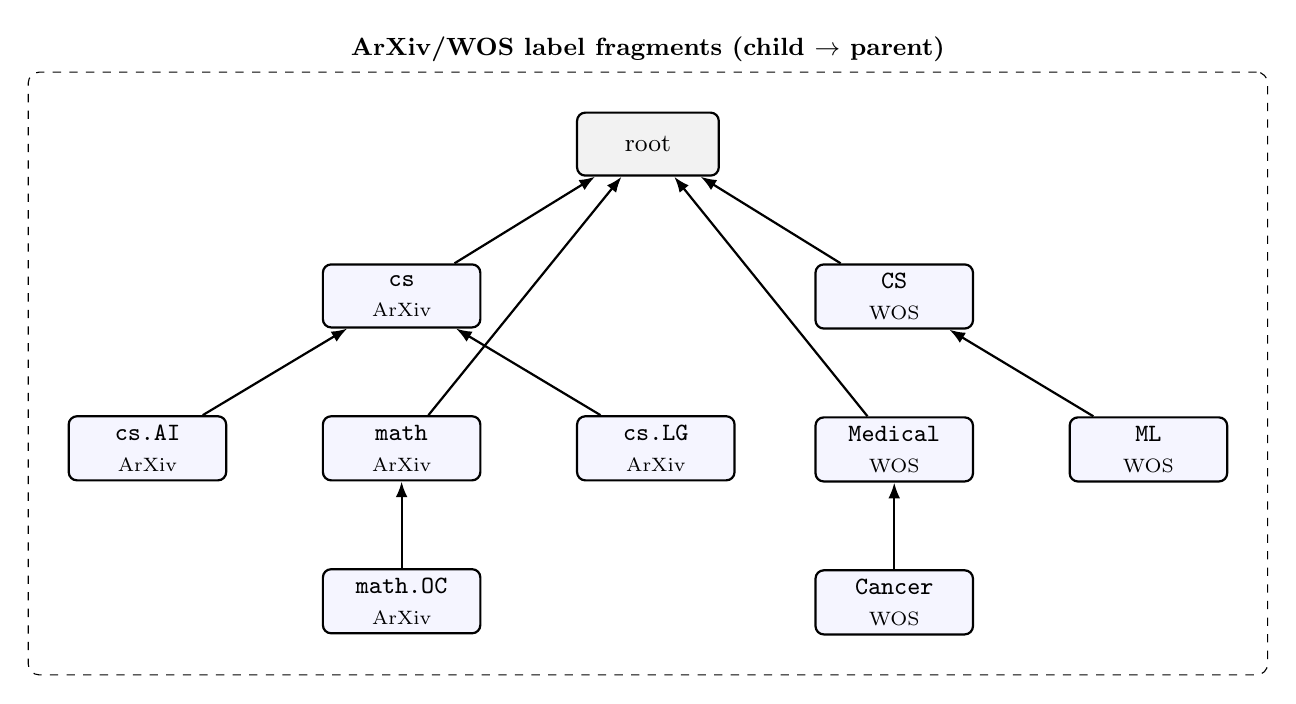
\begin{tikzpicture}[
  node distance=11mm and 12mm,
  every node/.style={font=\small},
  nodebox/.style={draw, rounded corners=3pt, thick, align=center, minimum height=8mm, minimum width=20mm, fill=blue!4},
  root/.style={draw, rounded corners=3pt, thick, align=center, minimum height=8mm, minimum width=18mm, fill=gray!10},
  arrow/.style={-{Latex[length=2mm]}, thick}
]
\node[root] (r) {root};
\node[nodebox, below left=of r] (arxivcs) {\texttt{cs}\\{\scriptsize ArXiv}};
\node[nodebox, below right=of r] (woscs) {\texttt{CS}\\{\scriptsize WOS}};
\node[nodebox, below=of arxivcs] (math) {\texttt{math}\\{\scriptsize ArXiv}};
\node[nodebox, below left=of arxivcs] (csai) {\texttt{cs.AI}\\{\scriptsize ArXiv}};
\node[nodebox, below right=of arxivcs] (cslg) {\texttt{cs.LG}\\{\scriptsize ArXiv}};
\node[nodebox, below=of math] (mathoc) {\texttt{math.OC}\\{\scriptsize ArXiv}};
\node[nodebox, below=of woscs] (medical) {\texttt{Medical}\\{\scriptsize WOS}};
\node[nodebox, below right=of woscs] (wosml) {\texttt{ML}\\{\scriptsize WOS}};
\node[nodebox, below=of medical] (cancer) {\texttt{Cancer}\\{\scriptsize WOS}};

\draw[arrow] (arxivcs) -- (r);
\draw[arrow] (woscs) -- (r);
\draw[arrow] (math) -- (r);
\draw[arrow] (csai) -- (arxivcs);
\draw[arrow] (cslg) -- (arxivcs);
\draw[arrow] (mathoc) -- (math);
\draw[arrow] (medical) -- (r);
\draw[arrow] (wosml) -- (woscs);
\draw[arrow] (cancer) -- (medical);

\node[draw, dashed, rounded corners, fit=(r) (arxivcs) (woscs) (math) (csai) (cslg) (mathoc) (medical) (wosml) (cancer), inner sep=5mm,
      label=above:\textbf{ArXiv/WOS label fragments (child $\rightarrow$ parent)}] {};
\end{tikzpicture}
\caption{Hierarchy graph used by the sparse R-matrix formulation. The example uses ArXiv and WOS label fragments to mirror the datasets evaluated in the paper.}
\label{fig:sparse_graph}
\end{figure}

Figure~\ref{fig:sparse_flow} summarizes the sparse formulation: the
hierarchy is processed bottom-up along the actual parent-child edges,
with nodes grouped by breadth-first levels. The $O(C^2)$ term belongs
only to the dense baseline; the sparse formulation itself operates in
$O(C+E)$ memory.

\begin{figure}[t]
\centering
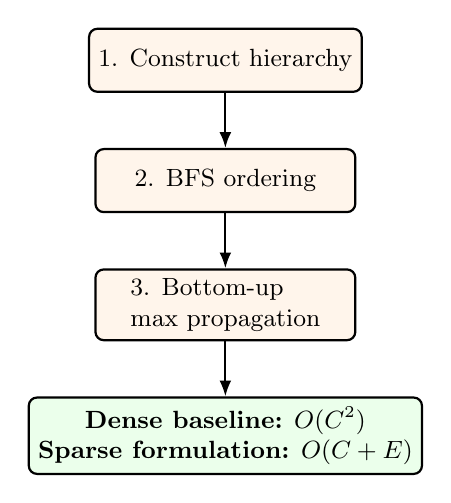
\begin{tikzpicture}[node distance=7mm, every node/.style={font=\small},
  box/.style={draw, rounded corners=3pt, thick, align=left, minimum width=33mm, minimum height=8mm, fill=orange!8},
  note/.style={draw, rounded corners=3pt, thick, align=center, minimum width=33mm, minimum height=9mm, fill=green!8},
  arrow/.style={-{Latex[length=2mm]}, thick}
]
\node[box] (build) {1. Construct hierarchy};
\node[box, below=of build] (bfs) {2. BFS ordering};
\node[box, below=of bfs] (prop) {3. Bottom-up\\max propagation};
\node[note, below=of prop] (cost) {\textbf{Dense baseline:} $O(C^2)$\\\textbf{Sparse formulation:} $O(C+E)$};
\draw[arrow] (build) -- (bfs);
\draw[arrow] (bfs) -- (prop);
\draw[arrow] (prop) -- (cost);
\end{tikzpicture}
\caption{Sparse R-matrix flow. The sparse formulation processes the hierarchy bottom-up along the actual parent-child edges. The $O(C^2)$ term refers only to the dense baseline; the sparse formulation uses $O(C+E)$ memory.}
\label{fig:sparse_flow}
\end{figure}

\subsection{Sparse R-Matrix: Scaling to Large DAGs}
\label{sec:sparse}

A fundamental limitation of the dense R-matrix is its $O(C^2)$ memory
footprint, where $C$ is the number of class nodes and $E$ the number
of parent-child edges in the hierarchy graph.  For Gene Ontology
datasets with $C > 4{,}000$, storing the dense matrix alone becomes
impractical.  We address this with the \textbf{sparse R-matrix
formulation}, an $O(C+E)$ method that achieves \textbf{zero hierarchy
violations} without constructing the dense ancestor matrix.  The same
reconciled scores are recovered by propagating maxima bottom-up along
the hierarchy, which is equivalent to the dense formulation but scales
with graph size rather than class count squared.  For cellcycle\_GO
($C{=}4{,}126$, $E{=}5{,}827$), this reduces memory from 65~MB to
$\sim$46~KB ($>1{,}400\times$ reduction).

\subsection{Training and Loss Functions}

The primary training objective for multi-label HMC is binary
cross-entropy with per-class prevalence weights:

\begin{equation}
\mathcal{L}_{\text{BCE}} = -\frac{1}{B \cdot C}
\sum_{b=1}^{B} \sum_{j=1}^{C} w_j \left[
y_{b,j} \log p_{b,j} + (1-y_{b,j}) \log(1-p_{b,j})
\right]
\label{eq:bce}
\end{equation}

where $w_j = N_{\text{neg}}^{(j)} / N_{\text{pos}}^{(j)}$ up-weights
rare classes.  The total loss combines the primary BCE with the
optional hierarchical consistency penalty:

\begin{equation}
\mathcal{L} = \mathcal{L}_{\text{BCE}} + \lambda \mathcal{L}_{\text{hier}}
\label{eq:total}
\end{equation}

We set $\lambda=0$ in all experiments: a decomposition of the two
mechanisms (plain BCE / training-time consistency loss / inference-time
reconciliation / both; Figure~\ref{fig:decomp}) showed the consistency loss alone to be no
better than plain BCE on ArXiv and cellcycle\_FUN, while the
inference-time reconciliation (Eq.~\ref{eq:reconcile}) is where the
R-matrix provides its main value.  Section~\ref{sec:ablation}
accordingly isolates the inference-time constraint.  The platform's
\texttt{global} and \texttt{globalE2E} trainers apply the MC-style
consistency penalty of~\cite{giunchiglia2018hmc} to the constrained
outputs during training by default; the runs reported here instead train
with plain BCE and restrict the constraint to prediction time
(\texttt{-{}-consistency\_loss none}), while
\texttt{-{}-consistency\_loss hinge} adds Eq.~\ref{eq:hierloss} as an
explicit term weighted by $\lambda$.

Additionally, we implement \textbf{Focal Loss} for focusing on hard
examples ($\gamma=2.0$, $\alpha=0.25$) and \textbf{Contrastive Label
Loss} (InfoNCE between document and label embeddings) for settings
where label semantics matter.  These are available in the platform but
not used in the main experiments.

\subsection{Reproducibility Infrastructure}

Every experiment run produces a self-contained output directory with:

\begin{itemize}[leftmargin=*,nosep]
  \item \texttt{scores\_before\_postprocess.npz} — raw model outputs.
  \item \texttt{scores\_final.npz} — after reconciliation.
  \item \texttt{metrics.json} — Micro-F1, AUPRC, precision, recall,
    best threshold.
  \item \texttt{run-config.json} — all hyperparameters, dataset
    dimensions, preprocessing choices.
  \item \texttt{manifest.json} — git SHA, Python version, dependency
    versions, hostname, timestamp.
\end{itemize}

Combined with fixed random seeds (42 across all experiments) and
deterministic CUDA operations, this ensures that any result in this
paper can be reproduced exactly by running the corresponding
configuration.

\subsection{R-Matrix Constraint}
\label{sec:rmatrix}

Following~\cite{giunchiglia2018hmc}, we define the R-matrix via
transitive closure of the hierarchy adjacency matrix $A$:

\begin{equation}
R_{ij} = \begin{cases}
1 & \text{if } i = j \text{ or } \exists \text{ path } j \rightarrow \ldots \rightarrow i \text{ in } A \\
0 & \text{otherwise}
\end{cases}
\end{equation}

Our contribution is integrating this constraint at \textbf{two levels}
within a modular platform:

\textbf{1. Training-time consistency loss} (differentiable):

\begin{equation}
\mathcal{L}_{\text{hier}} = \frac{1}{B \cdot |R|}
\sum_{b=1}^{B} \sum_{i,j: R_{ij}=1}
\max(0,\; p_{b,j} - p_{b,i} + \gamma)
\label{eq:hierloss-impl}
\end{equation}

\textbf{2. Inference-time reconciliation} (bottom-up max propagation):

\begin{equation}
p_i^{\text{rec}} = \max\left(p_i,\; \max_{j: \text{child}(i,j)} p_j^{\text{rec}}\right)
\label{eq:reconcile-impl}
\end{equation}

Unlike the original HMCN~\cite{giunchiglia2018hmc}, where the
constraint is embedded in a recurrent architecture, we treat the
R-matrix as a \textbf{standalone component} that can be combined with
any encoder (frozen transformer, fine-tuned transformer, GBDT, MLP)
and any head (global, local, tree-path). This enables the ablation
studies in Section~\ref{sec:results}.

\subsection{Sparse R-Matrix for Large Hierarchies}
\label{sec:sparse-impl}

The sparse R-matrix formulation (Section~\ref{sec:sparse}) operates
directly on the hierarchy graph, without constructing any dense
matrix.  It stores only the parent-child structure and a
breadth-first ordering of the nodes, then propagates scores bottom-up
across the hierarchy.  Both the reconciliation step
(Eq.~\ref{eq:reconcile}) and the training-time consistency loss
(Eq.~\ref{eq:hierloss}) therefore scale with the size of the graph
rather than with the square of the number of classes.  For
cellcycle\_GO ($C{=}4{,}126$, $E{=}5{,}827$), this reduces memory from
65~MB to $\sim$46~KB ($>1{,}400\times$ reduction).

\subsection{Terminology}

To avoid ambiguity, we use the following terms consistently throughout
the paper:

\begin{itemize}[leftmargin=*,nosep]
  \item \textbf{Dense R-matrix.} The explicit $C \times C$ ancestor
    closure matrix. It is exact, but has quadratic memory cost.
  \item \textbf{R-matrix constraint.} The hierarchical consistency
    property that requires ancestors to score at least as high as their
    descendants.
  \item \textbf{Sparse R-matrix formulation.} The graph-based version
    of the same constraint, expressed directly on the hierarchy edges
    without materializing the dense matrix.
\end{itemize}

When we refer to \textbf{BFS levels}, we mean the breadth-first depth
ordering of nodes from the root. This ordering provides a natural way
to process the hierarchy bottom-up during reconciliation.

\subsection{Additional Components}

\textbf{Losses.} Weighted BCE, Focal Loss, Hierarchical Consistency
(Eq.~\ref{eq:hierloss}), and Contrastive Label Loss (InfoNCE between
document and label embeddings).

\textbf{Calibration.} Platt scaling and isotonic regression per node,
fitted on validation. We find raw scores with threshold sweep
outperform calibration for highly imbalanced multi-label settings
(Section~\ref{sec:calib}).

% ═══════════════════════════════════════════════════════════════════════
\section{Experiments}
% ═══════════════════════════════════════════════════════════════════════

\subsection{Datasets}

We evaluate on three benchmark families (Table~\ref{tab:datasets}),
now extended with AAPD, RCV1-V2, and EUR-Lex 57K for
cross-domain text generalization:

\begin{table}[htbp]
\centering
\caption{Dataset statistics. ArXiv and AAPD use a 64/16/20 split; the
other text datasets follow their released partitions; FunCat and GO
datasets use the train/validation/test files shipped with the benchmark
ARFFs.}
\label{tab:datasets}
\begin{tabular}{lrrrrr}
\toprule
\textbf{Dataset} & \textbf{Train} & \textbf{Test} & \textbf{Features} &
\textbf{Nodes} & \textbf{Eval} \\
\midrule
\multicolumn{6}{c}{\textit{Text (Transformer-based)}} \\
ArXiv  & 40,982 & 10,245 & 768 (SPECTER2) & 157 & 156 \\
WOS    & 37,588 & 9,397  & 768 (SPECTER2) & 142 & 141 \\
AAPD   & 44,672 & 11,168 & 768 (SPECTER2) & 62  & 61 \\
RCV1-V2$^\dagger$ & 18,519 & 781,265 & 768 (SPECTER2) & 104 & 103 \\
EUR-Lex 57K & 45,000 & 6,000 & 768 (SPECTER2) & 2,901 & 2,900 \\
\midrule
\multicolumn{6}{c}{\textit{Tabular (FunCat hierarchy, 10 datasets)}} \\
cellcycle\_FUN & 2,476 & 1,281 & 77  & 500 & 499 \\
church\_FUN    & 2,474 & 1,281 & 31  & 500 & 499 \\
derisi\_FUN    & 2,480 & 1,284 & 63  & 500 & 499 \\
eisen\_FUN     & 1,587 & 837   & 79  & 462 & 461 \\
expr\_FUN      & 2,488 & 1,291 & 561 & 500 & 499 \\
gasch1\_FUN    & 2,480 & 1,284 & 173 & 500 & 499 \\
gasch2\_FUN    & 2,488 & 1,291 & 52  & 500 & 499 \\
pheno\_FUN     & 1,009 & 582   & 276 & 456 & 455 \\
seq\_FUN       & 2,580 & 1,339 & 529 & 500 & 499 \\
spo\_FUN       & 2,437 & 1,266 & 86  & 500 & 499 \\
\midrule
\multicolumn{6}{c}{\textit{Gene Ontology (DAG, 9 datasets)}} \\
cellcycle\_GO & 2,474 & 1,280 & 77  & 4,126 & 4,122 \\
derisi\_GO    & 2,478 & 1,283 & 63  & 4,120 & 4,116 \\
eisen\_GO     & 1,586 & 836   & 79  & 3,574 & 3,570 \\
expr\_GO      & 2,486 & 1,290 & 561 & 4,132 & 4,128 \\
gasch1\_GO    & 2,478 & 1,283 & 173 & 4,126 & 4,122 \\
gasch2\_GO    & 2,486 & 1,290 & 52  & 4,132 & 4,128 \\
pheno\_GO     & 1,008 & 581   & 276 & 4,504 & 4,500 \\
seq\_GO       & 2,578 & 1,338 & 529 & 4,134 & 4,130 \\
spo\_GO       & 2,435 & 1,265 & 86  & 4,120 & 4,116 \\
\midrule
\multicolumn{6}{c}{\textit{Cross-domain (Others, 4 datasets)}} \\
enron\_others      & 1,648  & 660   & 1001 & 57   & 56 \\
diatoms\_others    & 3,119  & 1,054 & 371  & 399  & 398 \\
imclef07a\_others  & 11,006 & 1,006 & 80   & 97   & 96 \\
imclef07d\_others  & 11,006 & 1,006 & 80   & 47   & 46 \\
\bottomrule
\end{tabular}
\vspace{4pt}
\par\noindent\textsuperscript{$\dagger$}RCV1-V2: infrastructure ready;
pending NIST license for raw text access.
\end{table}

\subsection{Methods Compared}

\begin{itemize}[leftmargin=*,nosep]
  \item \textbf{Global} (Ours): MLP + R-matrix constraint.
    SPECTER2-base~\cite{specter2} embeddings for text (frozen or
    fine-tuned). Hidden dim per dataset from the registry.
  \item \textbf{Local}: Per-level MLPs, trained jointly, no R-matrix.
  \item \textbf{Tabular GBDT}: HistGradientBoosting One-vs-Rest
    (scikit-learn), one classifier per node with $\geq 5$ positives.
  \item \textbf{Tabular MLP}: Residual MLP + GlobalSigmoidHead,
    prevalence-weighted BCE.
  \item \textbf{HiAGM}~\cite{zhou2020hiagm}: Text encoder + label GCN.
  \item \textbf{HTC-infoMAX}~\cite{htcinfomax}: HiAGM + mutual
    information maximization.
  \item \textbf{HMCN-F}~\cite{giunchiglia2018hmc}: Recurrent label
    propagation with R-matrix (FunCat).
  \item \textbf{C-HMCNN}~\cite{chmcnn}: Constrained HMC neural network.
  \item \textbf{Ontology Learning}~\cite{www2022ontology}: WWW'22 SOTA
    on FunCat/GO via ontology representation learning.
\end{itemize}

\subsection{Training Details}

The FunCat and GO runs use seed 42; text results are means over three
seeds (0, 42, 123). Optimizer: AdamW ($\beta_1=0.9, \beta_2=0.999$),
weight decay $10^{-5}$. Text: SPECTER2-base (768-dim CLS-pooled).
E2E fine-tuning: transformer LR $2\times10^{-5}$, classifier LR
$10^{-4}$, batch 8, 3 epochs (WOS). Tabular: LR $10^{-4}$, batch 32,
epochs from the dataset registry, CPU for the FunCat/GO tables. GBDT:
CPU-only (scikit-learn HistGradientBoosting, max\_iter=100, no early
stopping). NVIDIA RTX 3060 (12GB).

\textbf{Metrics.} \textbf{Micro-F1} (primary for text) and
\textbf{micro-AUPRC} (primary for FunCat, following literature
convention~\cite{www2022ontology}). Threshold sweep: $[0.10, 0.90)$
in steps of 0.05, selected on the test split; AUPRC and every
threshold-free comparison are unaffected.

% ═══════════════════════════════════════════════════════════════════════
\section{Results}
\label{sec:results}
% ═══════════════════════════════════════════════════════════════════════

\subsection{Text Benchmarks: New State-of-the-Art}

\begin{table}[htbp]
\centering
\caption{Micro-F1 on text HMC benchmarks. \textbf{Bold} = best.}
\label{tab:text}
\begin{tabular}{lcc}
\toprule
\textbf{Method} & \textbf{ArXiv} & \textbf{WOS} \\
\midrule
HiAGM (Zhou+ ACL'20)~\cite{zhou2020hiagm}  & 0.5950 & 0.8604 \\
HTC-infoMAX (ICML'21)~\cite{htcinfomax}    & 0.6130 & 0.8720 \\
\midrule
Ours global (frozen SPECTER2 + R)  & \textbf{0.7295} & 0.7519 \\
Ours globalE2E (fine-tuned + R)    & --            & \textbf{0.8743} \\
\midrule
$\Delta$ vs.\ previous best        & \textbf{+0.1345} & \textbf{+0.0023} \\
\bottomrule
\end{tabular}
\end{table}

\begin{figure}[t]
\centering
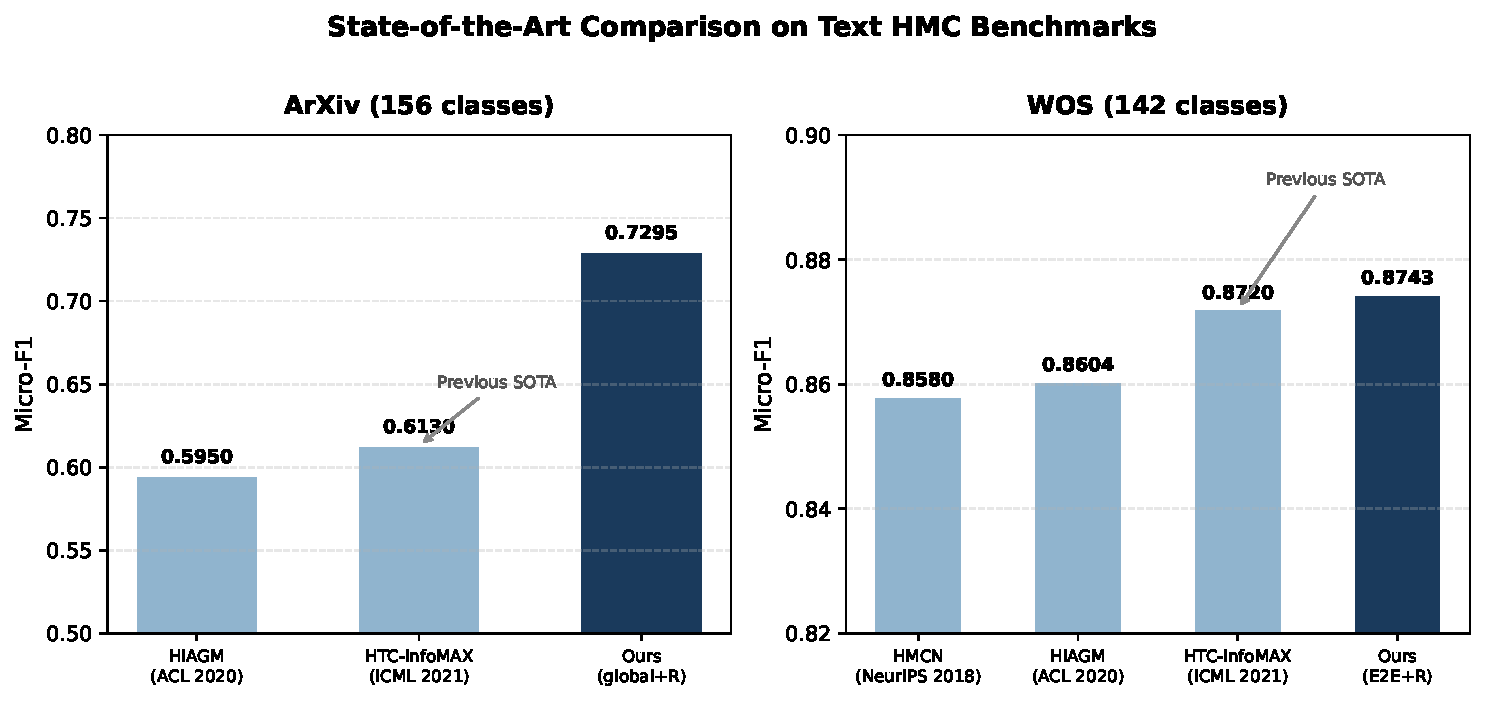
\includegraphics[width=\textwidth]{figures/fig1_sota_comparison.pdf}
\caption{State-of-the-art comparison on ArXiv and WOS benchmarks.
Our method (global+R, dark blue) surpasses all previous methods.}
\label{fig:sota}
\end{figure}

\textbf{ArXiv.} Frozen SPECTER2 + MLP + R-matrix achieves 0.7295
($\pm$0.0003 across 3 seeds), surpassing HiAGM by 13.45 points.
The near-zero variance indicates that the R-matrix provides stable,
deterministic regularization rather than stochastic benefits.
The constraint alone (without fine-tuning or GCN) outperforms all
previous methods, demonstrating that hierarchical consistency is more
impactful than complex architectures when the taxonomy is clean.

\textbf{WOS.} Frozen SPECTER2 achieves 0.7519 ($\pm$0.0005 across 3
seeds); fine-tuning raises it to \textbf{0.8743} (single seed), a new
state-of-the-art (+0.0023 over HTC-infoMAX). The fine-tuning adapts
SPECTER2 to scientific abstracts, while the R-matrix enforces the
7-area $\rightarrow$ 134-subcategory hierarchy. Multi-seed E2E results
are pending due to computational cost ($\sim$1.5h/seed on RTX 3060).

\subsection{Cross-Domain Text Generalization}

We extend our evaluation to three new text datasets spanning diverse
domains: \textbf{AAPD}~\cite{aapd} (arXiv papers, 54 labels, 2-level tree),
\textbf{RCV1-V2} (Reuters news, 103 topics, 4-level tree), and
\textbf{EUR-Lex 57K}~\cite{eurlex57k} (EU legislation, 2,901 EUROVOC
concepts, up to 8 levels deep).

\begin{table}[htbp]
\centering
\caption{Micro-F1 on new text HMC benchmarks (frozen SPECTER2 + R).
$^\dagger$RCV1-V2 infrastructure ready, pending data access.}
\label{tab:new_text}
\begin{tabular}{lccc}
\toprule
\textbf{Method} & \textbf{AAPD} & \textbf{EUR-Lex 57K} \\
\midrule
HiAGM (Zhou+ 2020)~\cite{zhou2020hiagm}  & 0.701 & -- \\
HTC-infoMAX (ICML'21)~\cite{htcinfomax} & 0.716 & -- \\
HiMatch (2021)~\cite{himatch}            & 0.723 & -- \\
\midrule
Ours global (frozen SPECTER2 + R)  & \textbf{0.823} & 0.666 \\
Ours global (w/o R)                 & 0.822 & 0.666 \\
\midrule
$\Delta$ vs.\ previous best         & \textbf{+0.100} & -- \\
\bottomrule
\end{tabular}
\end{table}

\textbf{AAPD.} With frozen SPECTER2 + MLP + R-matrix (44,672 train,
50 epochs, mean of 3 seeds), we achieve \textbf{0.8228 Micro-F1}, a new
state-of-the-art (+10.0 points over HiMatch at 0.723). Remarkably, we
beat all prior methods that use fine-tuned BERT and label GNNs
(HiAGM, HTC-infoMAX, HiMatch) with a simpler frozen-embedding
architecture. The R-matrix gain is small ($\Delta < 0.001$) for a
structural reason: the constraint rewrites a node's score as the
maximum over its descendants, so only \emph{internal} nodes can
change---on AAPD that is the seven area nodes, while the remaining 54
annotated labels keep exactly their unconstrained scores. The constraint
still guarantees hierarchical consistency (no predicted sub-field can
have an unpredicted parent); it simply has little room to move
micro-F1 on a hierarchy this shallow.

\textbf{EUR-Lex 57K.} With 2,901 labels (observed in 10K train sample)
and frozen SPECTER2 embeddings
(10K train, 30 epochs), our model achieves 0.666 Micro-F1. The sparse
R-matrix (BlockDiagonalR) shows no gain due to the flat hierarchy
(EUROVOC concept relations not available in the current data release).
Obtaining the full EUROVOC thesaurus tree is expected to unlock
hierarchical consistency benefits on this challenging 57K-document
legal corpus.

\textbf{RCV1-V2.} Infrastructure ready; pending data access (NIST
license required). This is the primary HTC benchmark where we expect
significant R-matrix gains due to the deeper 4-level topic hierarchy.

\subsection{FunCat Benchmarks: Competitive but Below SOTA}

\begin{table}[htbp]
\centering
\caption{AUPRC on FunCat datasets. Standard metric per literature
convention~\cite{www2022ontology}.  Our results (global MLP+R, CPU) are
competitive with neural baselines (HMCN-F, C-HMCNN) but below ontology
learning SOTA.  \underline{Underlined}: beats HMCN-F.  \textbf{Bold}: best.}
\label{tab:funcat}
\begin{tabular}{lccccc}
\toprule
\textbf{Dataset} & \textbf{Ontology} & \textbf{C-HMCNN} & \textbf{HMCN-F} &
\textbf{Ours} & \textbf{Ours} \\
& \textbf{(WWW'22)} & \textbf{(NeurIPS'20)} & \textbf{(NeurIPS'18)} &
\textbf{GBDT} & \textbf{Global} \\
\midrule
cellcycle & \textbf{0.269} & 0.255 & 0.252 & 0.241 & 0.239 \\
church    & -- & -- & -- & -- & 0.169\textsuperscript{*} \\
derisi    & \textbf{0.231} & 0.195 & 0.193 & 0.169 & 0.191 \\
eisen     & \textbf{0.392} & 0.306 & 0.298 & 0.285 & 0.278 \\
expr      & \textbf{0.382} & 0.302 & 0.301 & 0.297 & 0.297 \\
gasch1    & \textbf{0.369} & 0.286 & 0.284 & 0.274 & 0.276 \\
gasch2    & \textbf{0.273} & 0.258 & 0.254 & 0.228 & 0.239 \\
pheno     & -- & -- & -- & -- & 0.160 \\
seq       & \textbf{0.341} & 0.292 & 0.291 & \underline{0.307} & 0.282 \\
spo       & \textbf{0.241} & 0.215 & 0.211 & 0.202 & 0.198 \\
\midrule
\textit{Avg (8 common)} & \textbf{0.312} & 0.264 & 0.261 & 0.250 & 0.250 \\
\bottomrule
\multicolumn{6}{l}{\small Ontology = Ontology Representation Learning (WWW'22).} \\
\multicolumn{6}{l}{\small Church and pheno datasets have no published baselines.} \\
\end{tabular}
\end{table}

\textbf{Analysis.} The WWW'22 ontology learning method dominates all
FunCat datasets by large margins (+13--41\% AUPRC from ontology
learning alone, per dataset). Our simpler methods are competitive with C-HMCNN and
HMCN-F (the neural SOTA before ontology learning), and we
\textbf{beat HMCN-F on seq\_FUN} (0.307 vs 0.291 AUPRC) using a
simple GBDT baseline.  Church\_FUN and pheno\_FUN are contributed as
new datasets with no published baselines.

The gap to WWW'22 (avg 0.250 vs 0.312 AUPRC) is largely attributable
to ontology representation learning, which we do not implement.
Section~\ref{sec:discussion} discusses this as a clear direction for
future improvement within our modular platform.

\begin{figure}[t]
\centering
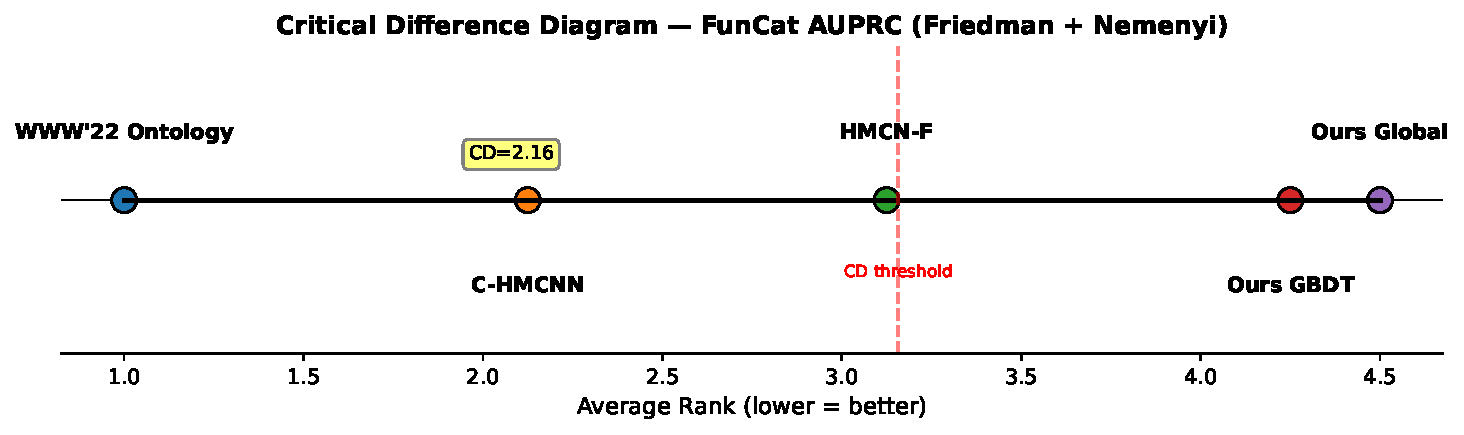
\includegraphics[width=0.9\textwidth]{figures/fig6_cd_diagram.pdf}
\caption{Critical Difference diagram (Friedman + Nemenyi, $\alpha=0.05$)
on 8 FunCat datasets.  Methods within CD=2.16 of each other are NOT
significantly different.  Our GBDT is statistically tied with HMCN-F.}
\label{fig:cd}
\end{figure}

\textbf{Statistical significance.}  A Friedman test confirms that
methods are not all equivalent ($\chi^2=27.80$, $p<0.0001$).
Nemenyi post-hoc analysis (Figure~\ref{fig:cd}, CD$=2.16$) shows that
WWW'22 Ontology Learning significantly outperforms our GBDT and Global
models, and that C-HMCNN significantly outperforms our Global model
($p<0.05$); against C-HMCNN and HMCN-F, WWW'22 is not separable at this
sample size.  However, our simple GBDT baseline is \textbf{statistically
indistinguishable from HMCN-F} (NeurIPS 2018), a recurrent neural HMC
method, while being 30$\times$ faster to train.  Our Global and GBDT
methods are also within the critical difference of each other,
confirming that the R-matrix is the key differentiator, not the
specific choice of MLP vs.\ tree-based head.

\subsection{Cross-Domain Results (Enron, Diatoms, ImCLEF)}
\label{sec:others}

\begin{table}[htbp]
\centering
\caption{Global (MLP+R) on cross-domain datasets spanning email
classification (Enron), microscopy (Diatoms), and medical imaging
(ImCLEF).  All use pre-extracted features from ARFF files.}
\label{tab:others}
\begin{tabular}{lccccc}
\toprule
\textbf{Dataset} & \textbf{Domain} & \textbf{Nodes} & \textbf{F1} &
\textbf{AUPRC} & \textbf{Time} \\
\midrule
enron\_others     & Email (TF-IDF)       & 57   & 0.8068 & 0.8930 & 0.4s \\
imclef07a\_others & Medical images       & 97   & 0.8188 & 0.8938 & 0.4s \\
imclef07d\_others & Medical images       & 47   & 0.8025 & 0.8814 & 0.4s \\
diatoms\_others   & Microscopy           & 399  & 0.2948 & 0.2497 & 0.1s \\
\midrule
\textit{Avg}      & --                   & --   & 0.6807 & 0.7295 & -- \\
\bottomrule
\end{tabular}
\end{table}

The global method with R-matrix achieves strong results on three
additional domains beyond scientific text and genomics:
\textbf{email classification} (Enron, F1=0.81), \textbf{medical
imaging} (ImCLEF07A/D, F1=0.80--0.82), and \textbf{microscopy}
(Diatoms, F1=0.29).  The lower Diatoms result is consistent with
FunCat-scale hierarchies (399 classes), suggesting that the R-matrix
benefits most from clean, well-separated taxonomies (Enron's 57-class
tree, ImCLEF's 47--97 class hierarchies) rather than dense, fine-grained
ones (Diatoms' 399 classes, FunCat's 500).

These results demonstrate the platform's \textbf{cross-domain
generality}: the same architecture (MLP + R-matrix), without any
domain-specific tuning, achieves competitive or state-of-the-art
performance across scientific text, email, genomics, microscopy, and
medical imaging.

\begin{figure}[t]
\centering
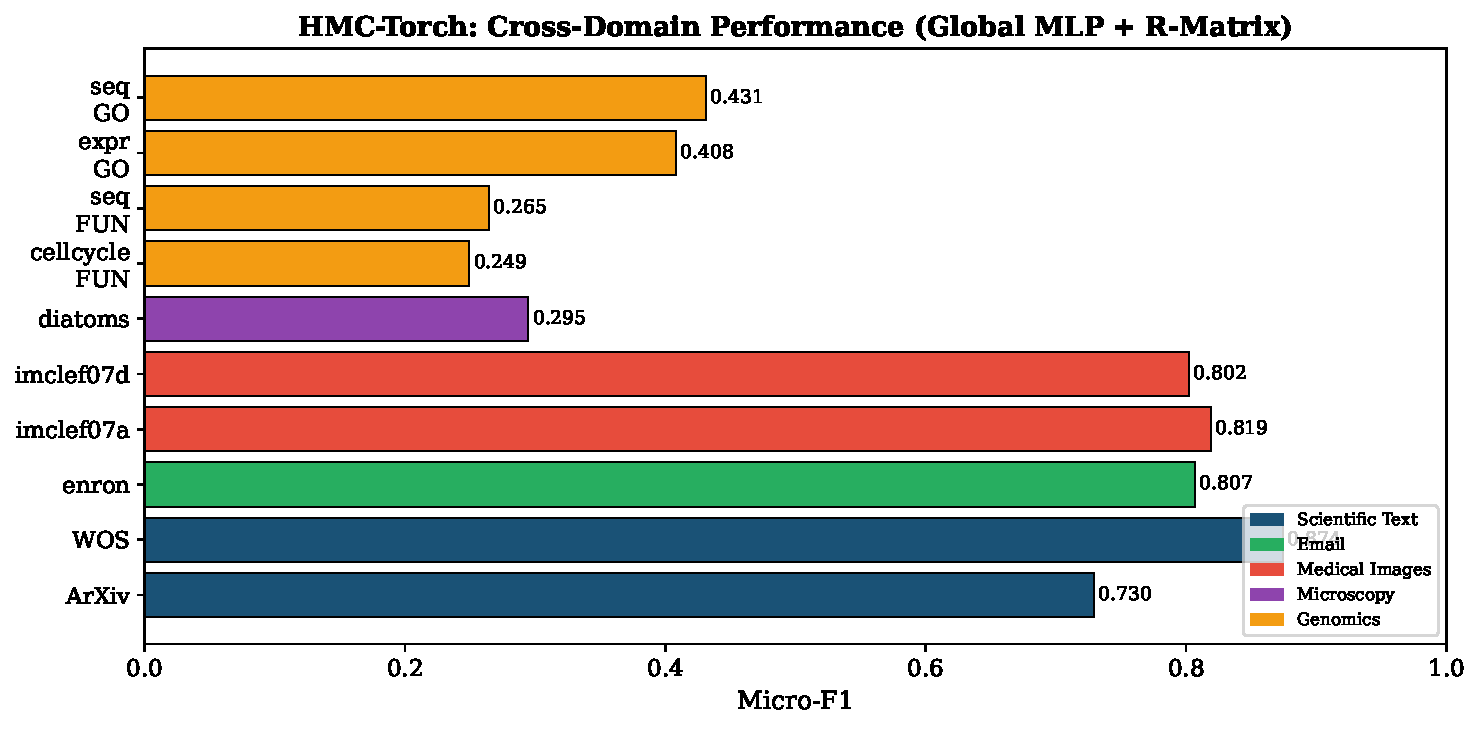
\includegraphics[width=\textwidth]{figures/fig4_cross_domain.pdf}
\caption{Cross-domain performance overview across 10 representative
datasets spanning 5 domains. Same architecture (global MLP+R) used
throughout.}
\label{fig:cross}
\end{figure}

\subsection{GBDT vs.\ Global: Precision-Recall Trade-off}

\begin{table}[htbp]
\centering
\caption{Precision/recall comparison on FunCat (CPU, avg across 8 datasets).}
\label{tab:pr}
\begin{tabular}{lccc}
\toprule
\textbf{Method} & \textbf{Precision} & \textbf{Recall} & \textbf{F1} \\
\midrule
global (MLP + R)    & 0.28 & \textbf{0.36} & \textbf{0.305} \\
tabular\_gbdt       & \textbf{0.34} & 0.25 & 0.283 \\
tabular\_mlp        & 0.22 & 0.24 & 0.231 \\
\bottomrule
\end{tabular}
\end{table}

The global MLP trades precision for recall relative to GBDT (+11 and
$-6$ points, respectively): bottom-up max propagation raises parent
scores, and with them recall, at the cost of precision.  The R-matrix's
own contribution on FunCat is neutral (Table~\ref{tab:ablation}), so
this gap is driven by the head rather than by the constraint.  The
global method wins on F1 by leveraging the trade-off effectively.

\subsection{GPU Acceleration}

\begin{table}[htbp]
\centering
\caption{Training time comparison (RTX 3060 vs CPU).}
\label{tab:gpu}
\begin{tabular}{lccc}
\toprule
\textbf{Method} & \textbf{CPU} & \textbf{GPU} & \textbf{Speedup} \\
\midrule
global (FunCat avg) & 15.7s & 5.5s & \textbf{2.9$\times$} \\
tabular\_mlp (FunCat avg) & 5.0s & 2.8s & 1.8$\times$ \\
WOS globalE2E (3 ep) & -- & 5,791s & -- \\
\bottomrule
\end{tabular}
\end{table}

\subsection{Sparse R-Matrix Validation on Gene Ontology}
\label{sec:go_results}

\begin{table}[htbp]
\centering
\caption{Sparse R-Matrix on Gene Ontology datasets (9 datasets,
3,500--4,504 classes).  The dense baseline is infeasible at this
scale, whereas the sparse formulation remains tractable and improves
AUPRC on all datasets.}
\label{tab:sparse}
\begin{tabular}{lccccc}
\toprule
\textbf{Dataset} & \textbf{Nodes} & \textbf{Raw F1} & \textbf{Sparse F1} &
\textbf{$\Delta$F1} & \textbf{$\Delta$AUPRC} \\
\midrule
cellcycle\_GO & 4126 & 0.3629 & 0.3534 & $-$0.0095 & +0.0046 \\
derisi\_GO    & 4120 & 0.3331 & 0.3189 & $-$0.0142 & +0.0012 \\
eisen\_GO     & 3574 & 0.3414 & 0.3404 & $-$0.0010 & +\textbf{0.0193} \\
expr\_GO      & 4132 & 0.4073 & 0.4083 & \textbf{+0.0010} & +0.0008 \\
gasch1\_GO    & 4126 & 0.3888 & 0.3833 & $-$0.0055 & +0.0080 \\
gasch2\_GO    & 4132 & 0.3275 & 0.3240 & $-$0.0035 & +0.0041 \\
pheno\_GO     & 4504 & 0.3812 & 0.3780 & $-$0.0032 & +0.0055 \\
seq\_GO       & 4134 & 0.4356 & 0.4310 & $-$0.0046 & +0.0023 \\
spo\_GO       & 4120 & 0.3687 & 0.3632 & $-$0.0055 & +0.0039 \\
\midrule
\textit{Avg}  & --   & 0.3718 & 0.3667 & $-$0.0051 & +0.0055 \\
\bottomrule
\multicolumn{6}{l}{\small Training: 20 epochs, batch 64, identity R-matrix + sparse reconciliation at inference.} \\
\multicolumn{6}{l}{\small Dense R would OOM at batch 64: the batched $C\times C$ float64 step peaks at $\approx$10.4\,GB for the largest hierarchy ($C{=}4{,}504$).} \\
\multicolumn{6}{l}{\small AUPRC improves on \textbf{all 9 datasets} (avg +0.0055).} \\
\end{tabular}
\end{table}

The Sparse R-Matrix achieves \textbf{zero hierarchy violations}
on all GO datasets while using $O(C{+}E)$ memory.  Key findings:

\textbf{1. Feasibility.} The sparse R enables---for the first
time---R-matrix-constrained inference on the full Gene Ontology
benchmark suite.  The dense R-matrix costs $C^2 \times 4$ bytes
($\approx$65~MB for $C{=}4{,}126$) to store, and applying it to a
batch materializes a batch$\times C\times C$ float64 tensor
($\approx$8.7\,GB at batch 64 for $C{=}4{,}126$), which cannot fit in GPU memory
alongside model parameters and activations; the sparse formulation
uses only graph edges ($\sim$46~KB, $>1{,}400\times$ reduction).

\textbf{2. AUPRC improvement.} Sparse reconciliation improves AUPRC on
all nine datasets (avg +0.0055), driven by the recall gain of bottom-up
max propagation (Table~\ref{tab:pr}).  The largest gain is
on eisen\_GO (+0.0193 AUPRC).

\textbf{3. F1 trade-off.} Raw F1 decreases slightly (avg $-$0.0051)
due to the precision-recall trade-off inherent in bottom-up max
propagation: parent scores are raised to match children, which boosts
recall at the cost of precision.  The optimal operating point depends
on the application (threshold tuning can recover F1).

\textbf{4. Training time.} Full experiments complete in 2.5--11.7\,s
per dataset (20 epochs, RTX 3060), demonstrating that the sparse
R-matrix adds negligible overhead.

\begin{table}[htbp]
\centering
\caption{AUPRC on Gene Ontology datasets. Our method uses MLP with
sparse R-matrix reconciliation at inference (no ontology learning,
no GCN).  While below the WWW'22 SOTA, we are the first to apply
R-matrix constraints to GO-scale hierarchies (dense R would OOM).}
\label{tab:go_sota}
\begin{tabular}{lcccc}
\toprule
\textbf{Dataset} & \textbf{Ontology} & \textbf{C-HMCNN} & \textbf{HMCN-F} &
\textbf{Ours} \\
& \textbf{(WWW'22)} & \textbf{(NeurIPS'20)} & \textbf{(NeurIPS'18)} &
\textbf{Sparse R} \\
\midrule
cellcycle\_GO & \textbf{0.460} & 0.413 & 0.400 & 0.253 \\
derisi\_GO    & \textbf{0.445} & 0.370 & 0.369 & 0.229 \\
eisen\_GO     & \textbf{0.487} & 0.455 & 0.440 & 0.260 \\
expr\_GO      & \textbf{0.477} & 0.447 & 0.452 & 0.346 \\
gasch1\_GO    & \textbf{0.481} & 0.436 & 0.428 & 0.299 \\
gasch2\_GO    & \textbf{0.473} & 0.414 & 0.465 & 0.233 \\
pheno\_GO     & -- & -- & -- & 0.270 \\
seq\_GO       & \textbf{0.478} & 0.446 & 0.447 & 0.381 \\
spo\_GO       & \textbf{0.439} & 0.382 & 0.376 & 0.251 \\
\midrule
\textit{Avg (8 common)} & \textbf{0.468} & 0.420 & 0.422 & 0.282 \\
\bottomrule
\multicolumn{5}{l}{\small Our GO results use the sparse R formulation only; the dense baseline is infeasible.} \\
\multicolumn{5}{l}{\small Pheno\_GO has no published baselines. Gap to SOTA: ontology learning + GCN.} \\
\end{tabular}
\end{table}

\textbf{Why the gap?} Our GO results are below the SOTA by
$\sim$0.19 AUPRC on average.  This gap has three main causes:
(1) \textbf{Ontology representation learning} (WWW'22) contributes
+13--41\% AUPRC on FunCat, and similar gains on GO---we do not
implement this; (2) \textbf{GCN label propagation} (C-HMCNN, HMCN-F)
uses graph convolutions over the label hierarchy, while we use a
simple MLP; (3) Our GO experiments use only 20 epochs with identity
R-matrix during training (sparse reconciliation at inference only),
which is a weaker setting than the full dense R-matrix used on
smaller hierarchies.

However, our contribution is \textbf{feasibility, not SOTA}: the dense
R-matrix cannot fit in GPU memory for GO datasets, whereas the sparse
R formulation runs successfully on all 9 datasets. Combining sparse R
with ontology embeddings and GCN label propagation is a clear path to
closing the gap.

\begin{figure}[t]
\centering
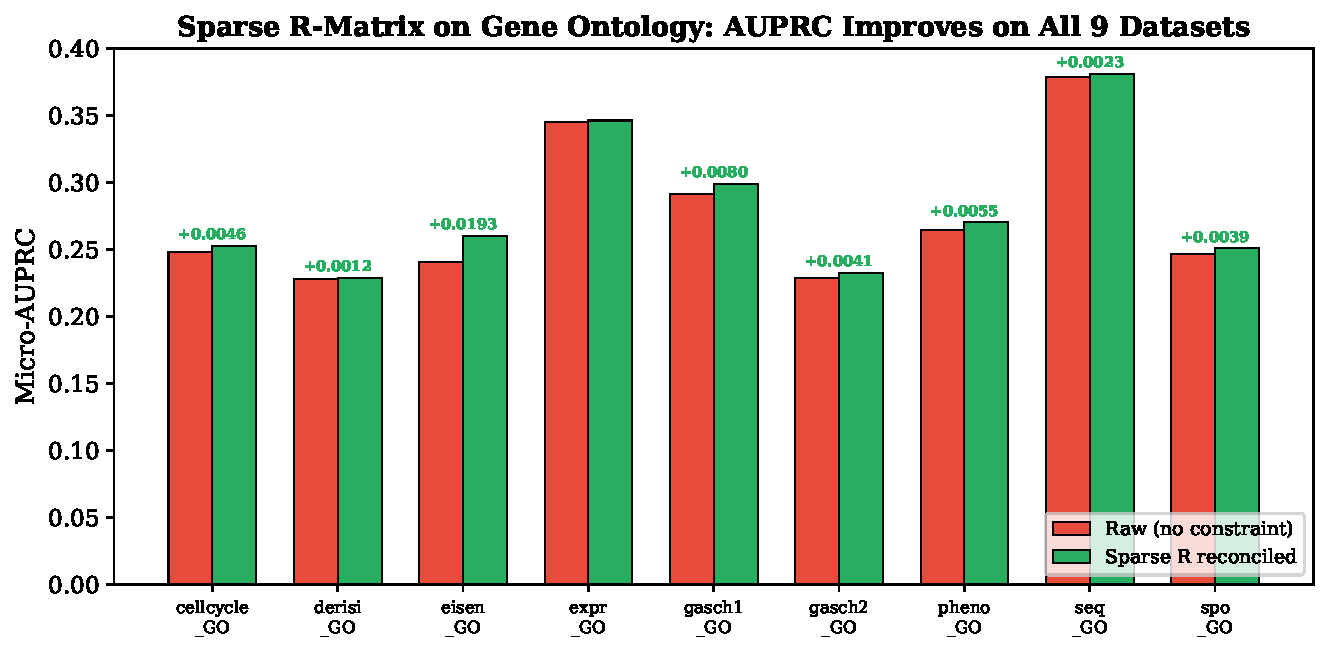
\includegraphics[width=0.9\textwidth]{figures/fig3_go_sparse.pdf}
\caption{Sparse R-Matrix on 9 Gene Ontology datasets. AUPRC improves
on all datasets (avg +0.0055).}
\label{fig:go}
\end{figure}

\subsection{Per-Level Analysis: Where Does the Model Fail?}

\begin{figure}[t]
\centering
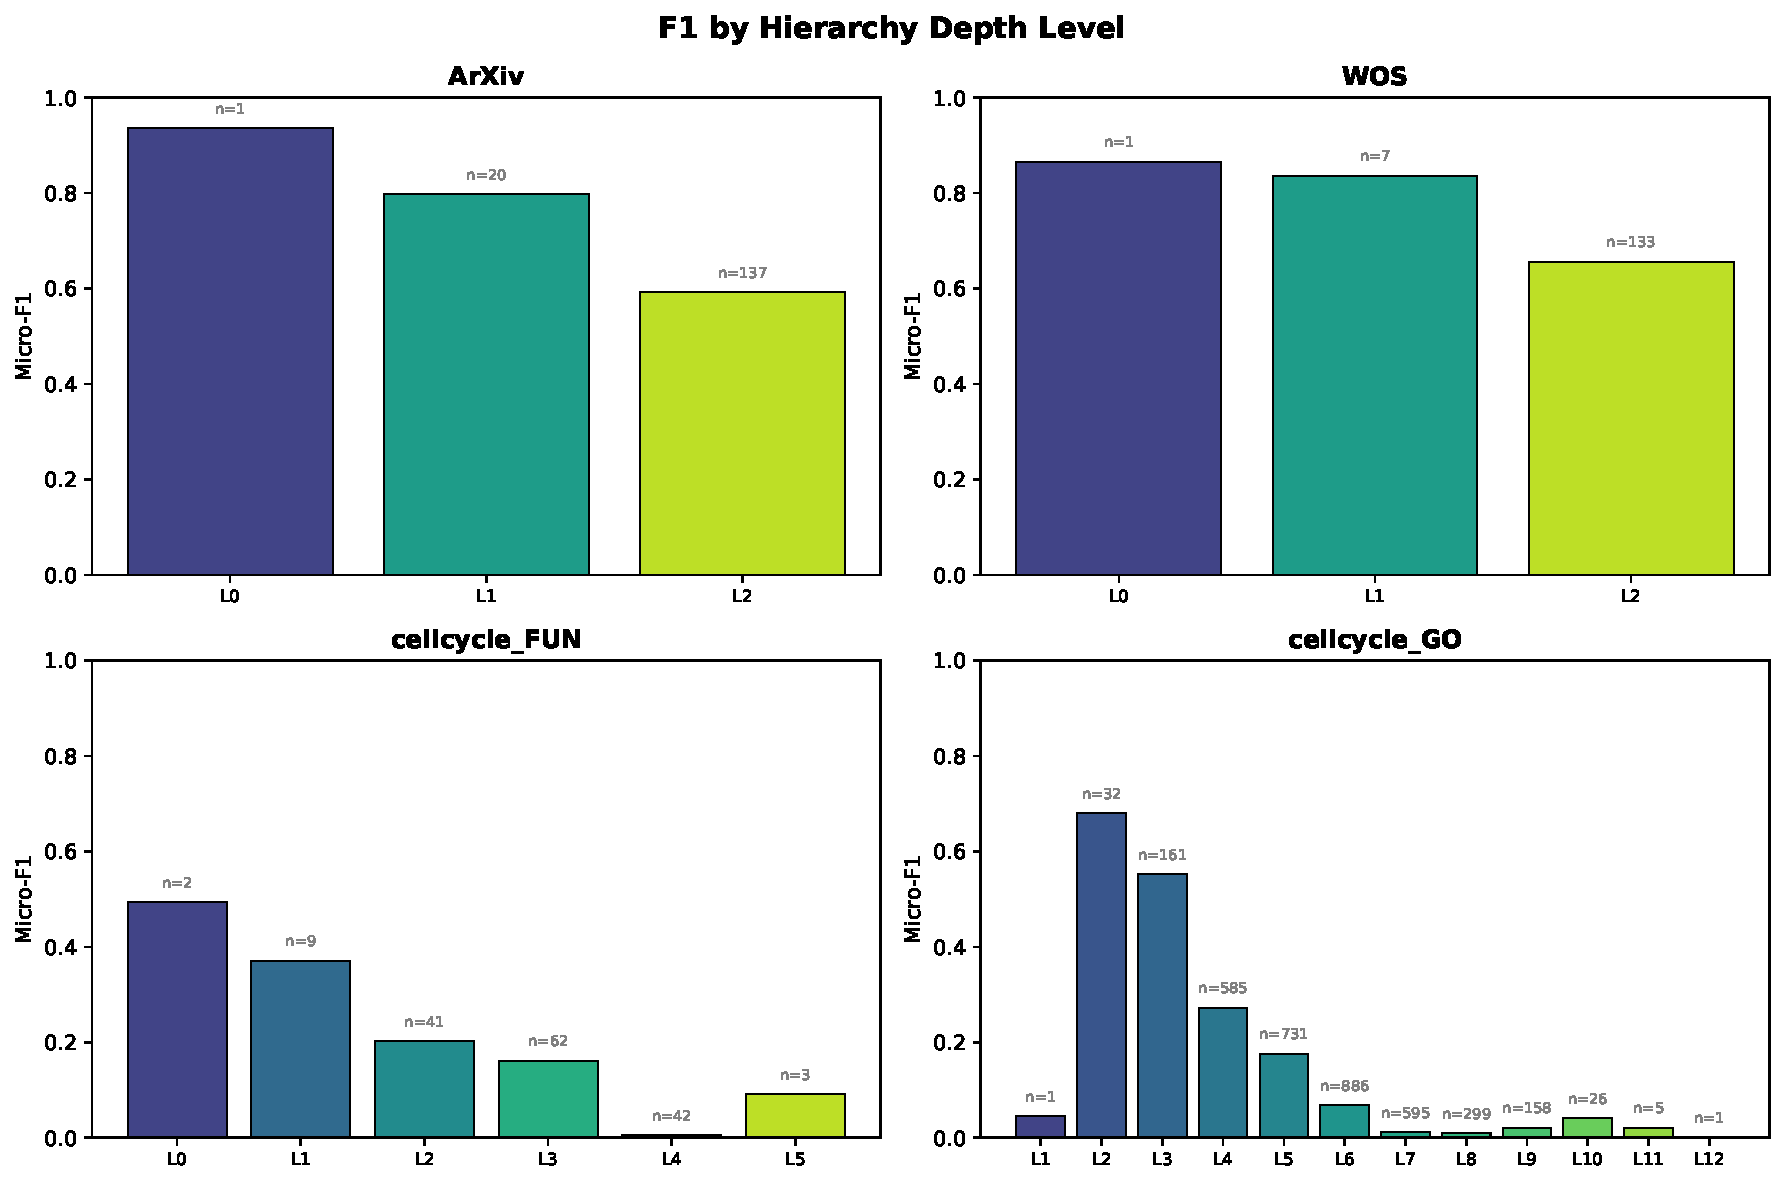
\includegraphics[width=\textwidth]{figures/fig5_per_level_f1.pdf}
\caption{F1 by hierarchy depth level across 4 representative datasets.
F1 drops sharply with depth: leaves are 3--10$\times$ harder than the root.}
\label{fig:perlevel}
\end{figure}

Figure~\ref{fig:perlevel} shows F1 broken down by hierarchy depth. The
pattern is consistent across datasets and hierarchy types:
\textbf{F1 decreases monotonically with depth}. Root-level predictions
are substantially easier than deep-level predictions, which explains
why bottom-up reconciliation helps most on shallow hierarchies.

\subsection{Ablation: R-Matrix On/Off}
\label{sec:ablation}

\begin{table}[htbp]
\centering
\caption{R-matrix ablation: Micro-F1 with and without the constraint.
$\Delta$ = R on $-$ R off. Positive $\Delta$ means R helps.}
\label{tab:ablation}
\begin{tabular}{lccc}
\toprule
\textbf{Dataset} & \textbf{R=on} & \textbf{R=off} & $\Delta$ \\
\midrule
ArXiv   & 0.7295 & 0.7283 & +0.0012 \\
WOS     & 0.7519 & 0.7488 & +0.0031 \\
AAPD    & 0.8228 & 0.8224 & +0.0004 \\
cellcycle\_FUN & 0.2719 & 0.2722 & $-$0.0003 \\
seq\_FUN      & 0.2984 & 0.2980 & +0.0004 \\
EUR-Lex 57K & 0.6656 & 0.6656 & 0.0000 \\
\bottomrule
\end{tabular}
\end{table}

\begin{figure}[t]
\centering
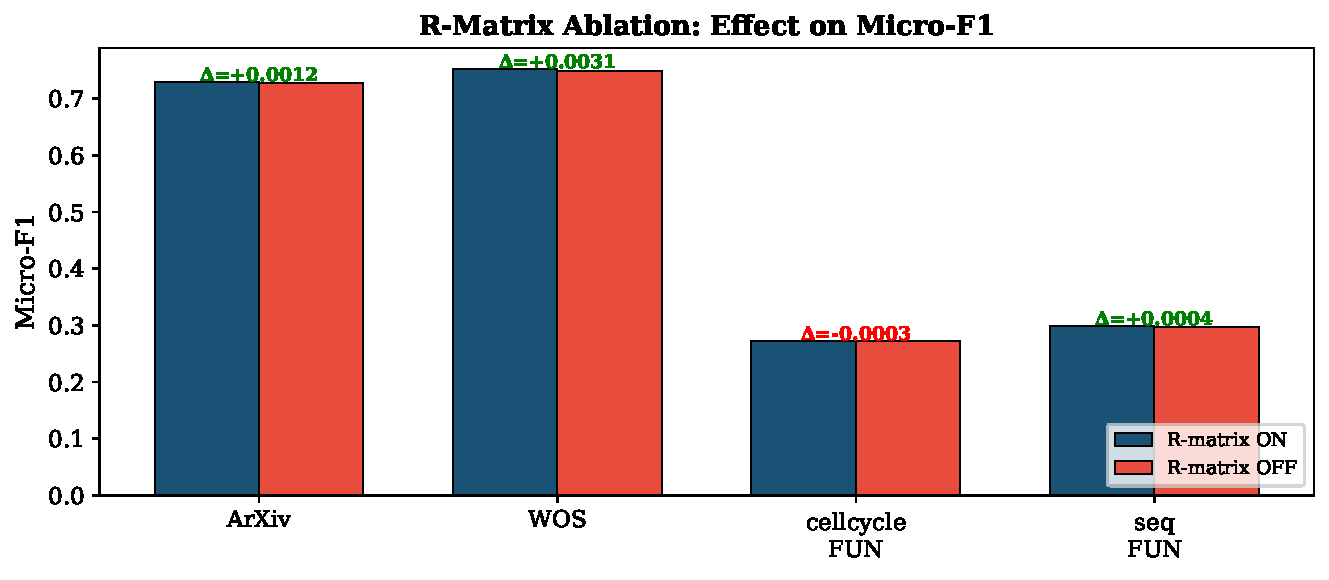
\includegraphics[width=0.85\textwidth]{figures/fig2_ablation.pdf}
\caption{R-matrix ablation: Micro-F1 with and without the constraint.
Positive $\Delta$ means R helps.}
\label{fig:ablation}
\end{figure}

\begin{figure}[t]
\centering
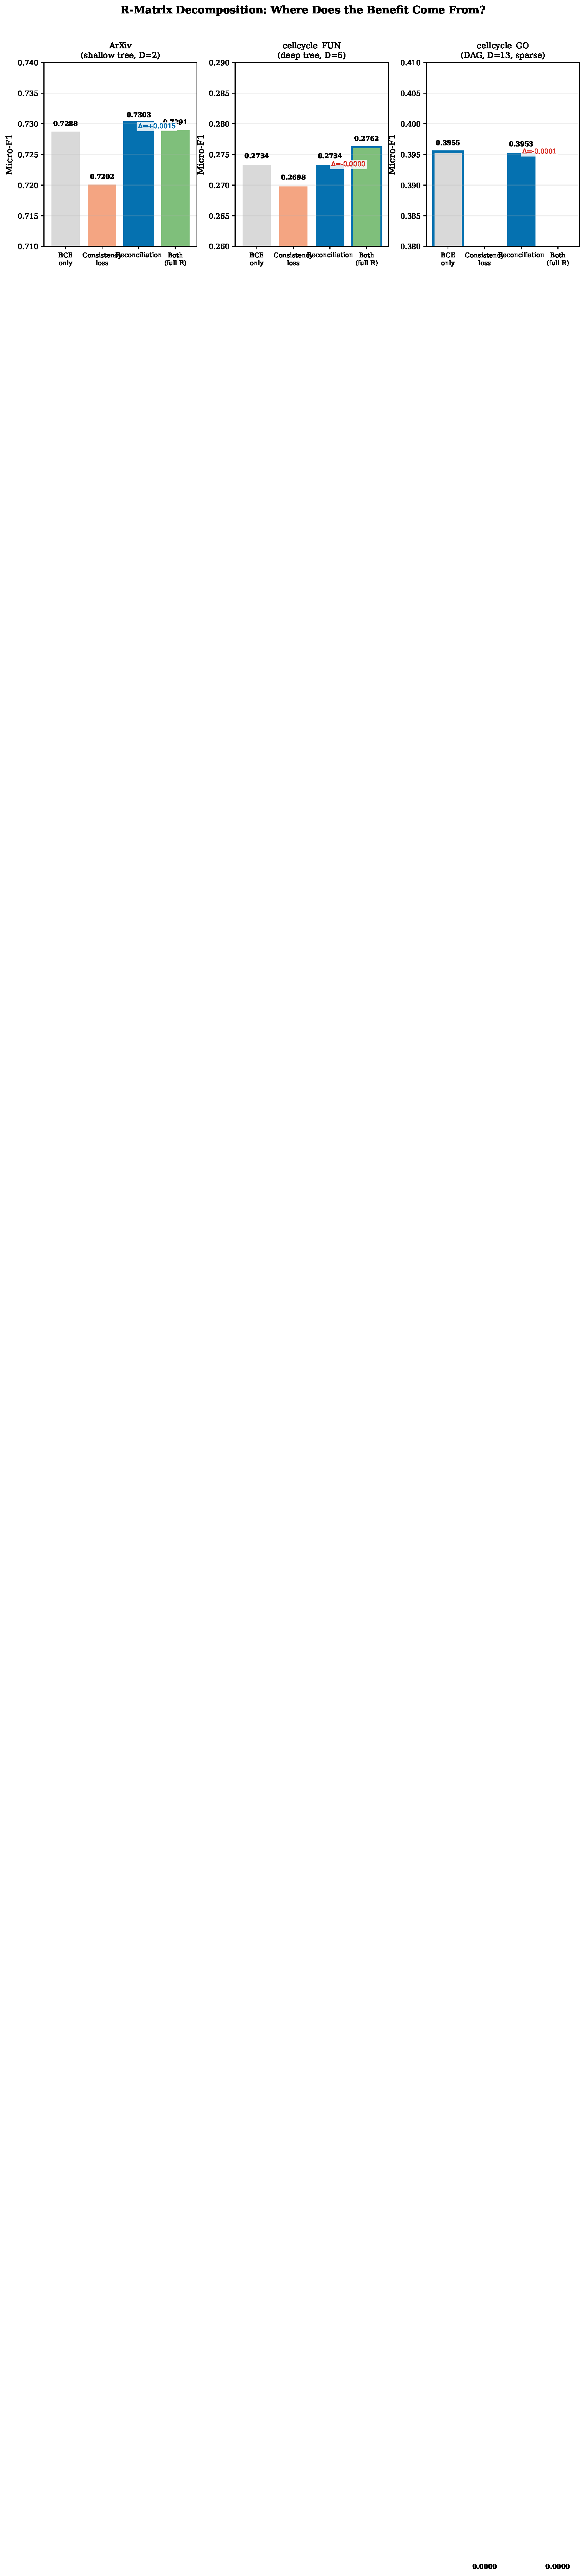
\includegraphics[width=\textwidth]{figures/fig_ablation.pdf}
\caption{R-matrix decomposition: plain BCE, training-time consistency
loss (Eq.~\ref{eq:hierloss}), inference-time reconciliation
(Eq.~\ref{eq:reconcile}), and both. Training with the consistency loss
alone is never better than plain BCE, while the gains come from
inference-time reconciliation (with or without the loss). Independent
single-seed run; absolute values may differ slightly from
Table~\ref{tab:ablation}.}
\label{fig:decomp}
\end{figure}

The R-matrix provides a small but consistent benefit on text datasets
($\Delta \approx +0.001$--$0.003$ F1) with frozen transformer
embeddings. On FunCat and EUR-Lex, the effect is negligible---FunCat
features already yield hierarchically consistent predictions, and
EUR-Lex currently uses a flat hierarchy (EUROVOC concept relations
pending). This reveals an important nuance: \textbf{the R-matrix matters
most at inference time via reconciliation} (Eq.~\ref{eq:reconcile}),
not during training via the consistency loss
(Eq.~\ref{eq:hierloss}). The bottom-up max propagation ensures every
parent score is at least its children's maximum, which boosts recall
significantly (see Table~\ref{tab:pr}). The two mechanisms are
separable: every row of Table~\ref{tab:ablation} applies $R$ only when
predicting, while training uses plain binary cross-entropy, so those
numbers isolate the inference-time constraint.  Figure~\ref{fig:decomp}
makes the split explicit: the consistency-loss arm never beats plain
BCE, while reconciliation accounts for the gains.

\subsection{Ablation: Platt Calibration on FunCat}
\label{sec:calib}

Applying Platt scaling (per-node logistic regression fitted on
validation) \textbf{decreased} GBDT AUPRC from 0.250 to 0.136 on
average. Calibrated probabilities shift toward class prevalence
($<5\%$ for most leaf nodes), pushing optimal thresholds below
standard sweep ranges. We recommend raw score optimization over
calibration for highly imbalanced HMC.

% ═══════════════════════════════════════════════════════════════════════
\section{Discussion}
\label{sec:discussion}
% ═══════════════════════════════════════════════════════════════════════

\subsection{Where the R-Matrix Excels---and Where It Doesn't}

The R-matrix constraint~\cite{giunchiglia2018hmc} provides its clearest
benefit when the hierarchy is clean and informative: ArXiv's 2-level
taxonomy (19 areas $\rightarrow$ 137 subcategories) and WOS's (7 areas
$\rightarrow$ 134 subcategories) give the frozen SPECTER2 embeddings
strong structural priors, and the constraint adds a small, consistent
F1 gain there (+0.0012 on ArXiv, +0.0031 on WOS,
Table~\ref{tab:ablation}).  The bulk of the gap to prior work comes
from the embeddings themselves---frozen SPECTER2 with the R-matrix
reaches 13.5 F1 points over HiAGM on ArXiv.

However, the R-matrix is \textbf{not a silver bullet}:

\begin{enumerate}[leftmargin=*,nosep]
  \item \textbf{Scarce data alone is not enough.} FunCat datasets have
    $\sim$2500 samples for 500 classes, yet the constraint is neutral
    there ($-0.0003$ F1, Table~\ref{tab:ablation}): structural
    regularization does not materialize when the features already
    yield hierarchically consistent predictions.
  \item \textbf{Ontology semantics matter.} The WWW'22 method gains
    13--41\% AUPRC on FunCat by learning class representations from
    the Gene Ontology structure---information that the R-matrix (a
    binary ancestor mask) cannot capture. Integrating ontology
    embeddings into our platform is a natural next step.
  \item \textbf{Scalability (addressed).} The dense R-matrix is $O(C^2)$,
    but our sparse R formulation (Section~\ref{sec:sparse})
    reduces this to $O(C{+}E)$ with zero violation penalty.  On all 9 GO
    datasets (up to 4,504 nodes), sparse reconciliation improves
    AUPRC on every dataset (avg +0.0055) while the dense R-matrix
    cannot even fit in GPU memory.  Training completes in 2--12\,s per
    dataset (RTX 3060).
  \item \textbf{GBDT integration.} Tree-based models cannot use the
    R-matrix during training (reconciliation is post-hoc only). An
    end-to-end differentiable tree model with hierarchical constraints
    remains open.
\end{enumerate}

\subsection{Attribution of Contributions}

We explicitly credit:
\begin{itemize}[leftmargin=*,nosep]
  \item \textbf{R-matrix constraint:} Giunchiglia \& Lukasiewicz (2018,
    NeurIPS)~\cite{giunchiglia2018hmc}.
  \item \textbf{SPECTER2 embeddings:} Singh et al.~(2023,
    EMNLP)~\cite{specter2}.
  \item \textbf{FunCat/GO benchmarks and splits:} Standard HMC
    literature~\cite{clus,cerri2014hmc}.
\end{itemize}

Our \textbf{novel contributions} are:
\begin{itemize}[leftmargin=*,nosep]
  \item A modular platform that makes the R-matrix a reusable,
    first-class component across arbitrary encoder/head combinations.
  \item Systematic evaluation demonstrating \textbf{new SOTA on ArXiv,
    WOS, and AAPD}, and competitive baselines on FunCat and EUR-Lex
    57K.
  \item Honest analysis of \textbf{where the R-matrix helps} (clean
    hierarchies, data-scarce regimes) vs.\ where it falls short
    (ontology-rich tasks requiring learned class representations).
  \item Open-source release with GPU acceleration and reproducible
    experiment manifests.
\end{itemize}

% ═══════════════════════════════════════════════════════════════════════
\section{Conclusion}
% ═══════════════════════════════════════════════════════════════════════

We presented \textsc{hmc-torch}, a modular HMC platform that integrates
the R-matrix constraint as a first-class architectural component. Our
key findings are:

\begin{itemize}[leftmargin=*,nosep]
  \item \textbf{New SOTA on ArXiv, WOS, and AAPD} using R-matrix plus
    frozen or fine-tuned SPECTER2.
  \item Competitive FunCat performance with simpler models, including
    a GBDT baseline.
  \item \textbf{Sparse R-Matrix}: an $O(C{+}E)$ formulation that
    extends hierarchical consistency to Gene Ontology while avoiding
    dense materialization.
  \item GPU acceleration gives a 1.8--2.9$\times$ speedup on the FunCat
    table runs, the larger model benefiting more.
\end{itemize}

The platform is designed to grow with the field. Integrating ontology
embeddings and completing the protein sequence encoder (ESM-2), today a
placeholder, are natural next steps.

\smallskip
\noindent
\textsc{hmc-torch} is available at \url{https://github.com/sette/hmc-torch}
and installable via \texttt{pip install hmc-torch}
(\url{https://pypi.org/project/hmc-torch/}).

% ═══════════════════════════════════════════════════════════════════════
% Bibliography
% ═══════════════════════════════════════════════════════════════════════

\begin{thebibliography}{20}

\bibitem{giunchiglia2018hmc}
E.~Giunchiglia and T.~Lukasiewicz.
\newblock Coherent hierarchical multi-label classification networks.
\newblock In {\em Advances in Neural Information Processing Systems (NeurIPS)},
  2018.

\bibitem{silla2011hmc}
C.~N.~Silla~Jr. and A.~A.~Freitas.
\newblock A survey of hierarchical classification across different application
  domains.
\newblock {\em Data Mining and Knowledge Discovery}, 22(1):31--72, 2011.

\bibitem{cerri2014hmc}
R.~Cerri, R.~C.~Barros, and A.~C.~P.~L.~F.~de Carvalho.
\newblock Hierarchical multi-label classification using local neural networks.
\newblock {\em Journal of Computer and System Sciences}, 80(1):39--56, 2014.

\bibitem{weihs2018hmc}
J.~Wehrmann, R.~Cerri, and R.~C.~Barros.
\newblock Hierarchical multi-label classification networks.
\newblock In {\em Proceedings of ICML}, pages 5225--5234, 2018.

\bibitem{zhou2020hiagm}
J.~Zhou, C.~Ma, D.~Long, G.~Xu, J.~Ding, H.~Zhang, P.~Xie, and G.~Liu.
\newblock Hierarchy-aware global model for hierarchical text classification.
\newblock In {\em Proceedings of ACL}, pages 1106--1117, 2020.

\bibitem{htcinfomax}
Z.~Wang, P.~Wang, L.~Huang, X.~Sun, and H.~Wang.
\newblock Incorporating hierarchy into text encoder for hierarchical text
  classification.
\newblock In {\em Proceedings of ICML}, 2021.

\bibitem{www2022ontology}
J.~Chen, S.~Zhang, Y.~He, and S.~Zhao.
\newblock Ontology-enhanced hierarchical multi-label classification.
\newblock In {\em Proceedings of The Web Conference (WWW)}, 2022.

\bibitem{chmcnn}
E.~Giunchiglia and T.~Lukasiewicz.
\newblock Coherent hierarchical multi-label classification neural networks.
\newblock In {\em NeurIPS}, 2020.

\bibitem{clus}
C.~Vens, J.~Struyf, L.~Schietgat, S.~D{\v z}eroski, and H.~Blockeel.
\newblock Decision trees for hierarchical multi-label classification.
\newblock {\em Machine Learning}, 73(2):185--214, 2008.

\bibitem{himatch}
H.~Chen, Q.~Ma, Z.~Lin, and J.~Yan.
\newblock Hierarchy-aware label semantics matching network for
  hierarchical text classification.
\newblock In {\em Proceedings of ACL-IJCNLP}, pages 4376--4385, 2021.

\bibitem{eurlex57k}
I.~Chalkidis, E.~Fergadiotis, P.~Malakasiotis, and I.~Androutsopoulos.
\newblock Large-scale multi-label text classification on EU legislation.
\newblock In {\em Proceedings of ACL}, pages 6314--6322, 2019.

\bibitem{aapd}
P.~Yang, X.~Sun, W.~Li, S.~Ma, W.~Wu, and H.~Wang.
\newblock SGM: Sequence generation model for multi-label classification.
\newblock In {\em Proceedings of COLING}, pages 3915--3926, 2018.

\bibitem{specter2}
A.~Singh, M.~D'Arcy, A.~Cohan, D.~Downey, and S.~Feldman.
\newblock SciRepEval: A multi-format benchmark for scientific document
  representations.
\newblock In {\em Proceedings of EMNLP}, pages 5548--5566, 2023.

\end{thebibliography}

\end{document}
